\begin{problem}{Þyngdarflokkur}{Inn}{Út}{~}{~}

	\begin{wrapfigure}{r}{0.30\textwidth}
		\vspace{-25pt}
		\begin{center}
			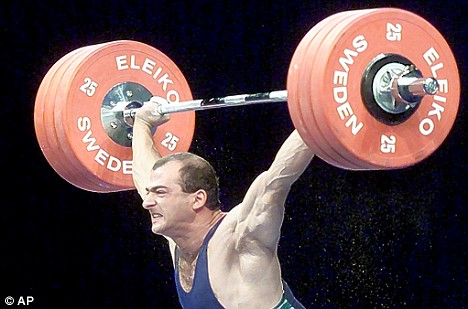
\includegraphics[scale=0.30]{../Thyngdarflokkur/heavyLifting.jpg}
		\end{center}
		\vspace{-30pt}
	\end{wrapfigure}

	Verið er að undirbúa kraftlyftingakeppni sem haldin verður á næstunni. Keppendum er skipt upp í þrjá þyngdarflokka; léttvigt, millivigt og þungavigt. Eftirfarandi sýnir hvernig keppendunum er skipt upp eftir þyngd:

	\begin{center}
		\hspace{-10pt}
		\begin{tabular}{lc}
			\hline
			Flokkur & Þyngd (kg) \\
			\hline
			Léttvigt & $< 60$ \\
			Millivigt & $\geq 60$ og $\leq 90$ \\
			Þungavigt & $> 90$ \\
			\hline
		\end{tabular}
	\end{center}

	Skrifið forrit sem les inn nöfn og þyngd keppenda, og skrifar út hvaða flokki hver keppandi tilheyrir.

	\Input
		Á fyrstu línu er heiltalan $1 \leq T \leq 100$, sem táknar fjölda prófunartilvika sem fylgja. Hvert prófunartilvik samanstendur af tveimur línum. Fyrri línan inniheldur nafn keppandans, og seinni línan inniheldur kommutölu sem táknar þyngd keppandans í kílógrömmum.

	\Output
		Fyrir hvert prófunartilvik á að skrifa út eina línu. Ef keppandinn tilheyrir léttvigt á línan að innihalda "`\textit{nafn} \texttt{competes in lightweight}"'. Ef keppandinn tilheyrir millivigt á línan að innihalda "`\textit{nafn} \texttt{competes in middleweight}"'. Ef keppandinn tilheyrir þungavigt á línan að innihalda "`\textit{nafn} \texttt{competes in heavyweight}"'.

	\Examples

		\begin{example}
			\exmp{
4
Bob
95.5
Georg
50.0
David
90.0
John Doe
90.3
			}{
Bob competes in heavyweight
Georg competes in lightweight
David competes in middleweight
John Doe competes in heavyweight
}%
		\end{example}

\end{problem}